\section{Évaluation des extensions proposées}\label{sec:contribs:perf_eval}

Nous avons évalué les différentes améliorations proposées dans les sections~\ref{sec:openmp:langage} et~\ref{sec:openmp:runtime} sur les machines idchire et brunch, décrites en détails dans la section~\ref{sec:contribs:machines}.

La section suivante décrit les différents logiciels que nous avons utilisé pour nos expériences, ainsi que les modifications apportées le cas échéant ; et la section~\ref{sec:contribs:perf_eval:resultats} aborde point par point les extensions proposées.
Enfin la section~\ref{sec:contribs:perf_eval:libkomp} discute de l'application de nos idées dans un support exécutif différent, avec également une évaluation de performances.


\subsection{Logiciels}

Les logiciels utilisés pour nos expériences peuvent être divisé en trois catégories~:
\begin{itemize}
  \item Les applications utilisées
  \item Les supports exécutifs
  \item Les bibliothèques externes
\end{itemize}

Les applications et les supports exécutifs utilisées ont pu subire quelques modifications afin d'incorporer les modifications d'OpenMP proposées.
Ces changements sont décrits ci-dessous.
Nous n'avons effectué aucune modification aux bibliothèques externes, mais il est important de faire un point dessus, étant donné qu'une partie des performances peut en dépendre.

\subsubsection{Applications utilisées}

Les applications utilisées pour ces expériences proviennent des KASTORS\footnote{https://gitlab.inria.fr/openmp/kastors, branche 'affinity'}.

Nous avons ajouté une clause \emph{affinity} dans certaines applications~: dans le cas des applications d'algèbre linéaire, les tâches de calculs dépendent d'un ou plusieurs blocs de données. Nous avons ajouté une affinité entre chaque tâche et les données qu'elle écrit.
Dans le cas des applications de type stencil, nous avons ajouté une affinité vers un cœur précis pour les tâches successives.


\subsubsection{Supports exécutifs}


\paragraph{XKAAPI}~: nous avons implémentés les trois types d'extensions proposés dans la section~\ref{sec:openmp:runtime}, à savoir les différentes stratégies de distribution des données, les stratégies de sélection lors du vol de travail, et les stratégies de placement des tâches prêtes.
Ces modifications ont été rassemblées dans une version spécifique de XKAAPI~\footnote{https://scm.gforge.inria.fr/anonscm/git/kaapi/xkaapi.git, branche 'public/europar2016'}.


Nous avons pris comme base de comparaison les supports exécutifs fournis avec les compilateurs existant au moment de nos propositions.

\paragraph{GCC/libGOMP}~: nous avons utilisé la version 5.2.0 comme référence, sans y apporter de modification.

\paragraph{Clang/libOMP}~: nous avons utilisé la version 3.8. Bien que le support exécutif (libOMP) n'ait pas été modifié, le compilateur (Clang) a subit des modifications afin de supporter les clauses décrites dans la section~\ref{sec:openmp:langage}.

\subsubsection{Bibliothèques externes}

\paragraph{BLAS} : les applications d'algèbre linéaire des KASTORS dépendent de la bibliothèque BLAS.
Pour les expériences effectuées dans la section~\ref{sec:contribs:perf_eval:resultats}, nous avons utilisé la bibliothèque OpenBLAS~2.15 pour fournir les noyaux de calculs de base.


\paragraph{hwloc} : cette bibliothèque fournie les informations sur la hiérarchie de la machine, ainsi que des fonctions d'allocation de mémoire selon différentes politique (voir section~\ref{sec:context:os:lib}). Nous avons utilisé la version 1.11.0.

\paragraph{numactl} : nous avons utilisé \emph{numactl} pour certaines courbes de référence. \emph{numactl} est fourni par libNUMA ; nous avons utilisé la version par défaut fourni par le fabricant de la machine.


\subsection{Résultats}\label{sec:contribs:perf_eval:resultats}

\subsubsection{Impact de la distribution des données}

\begin{figure}[ht]
  \centering
  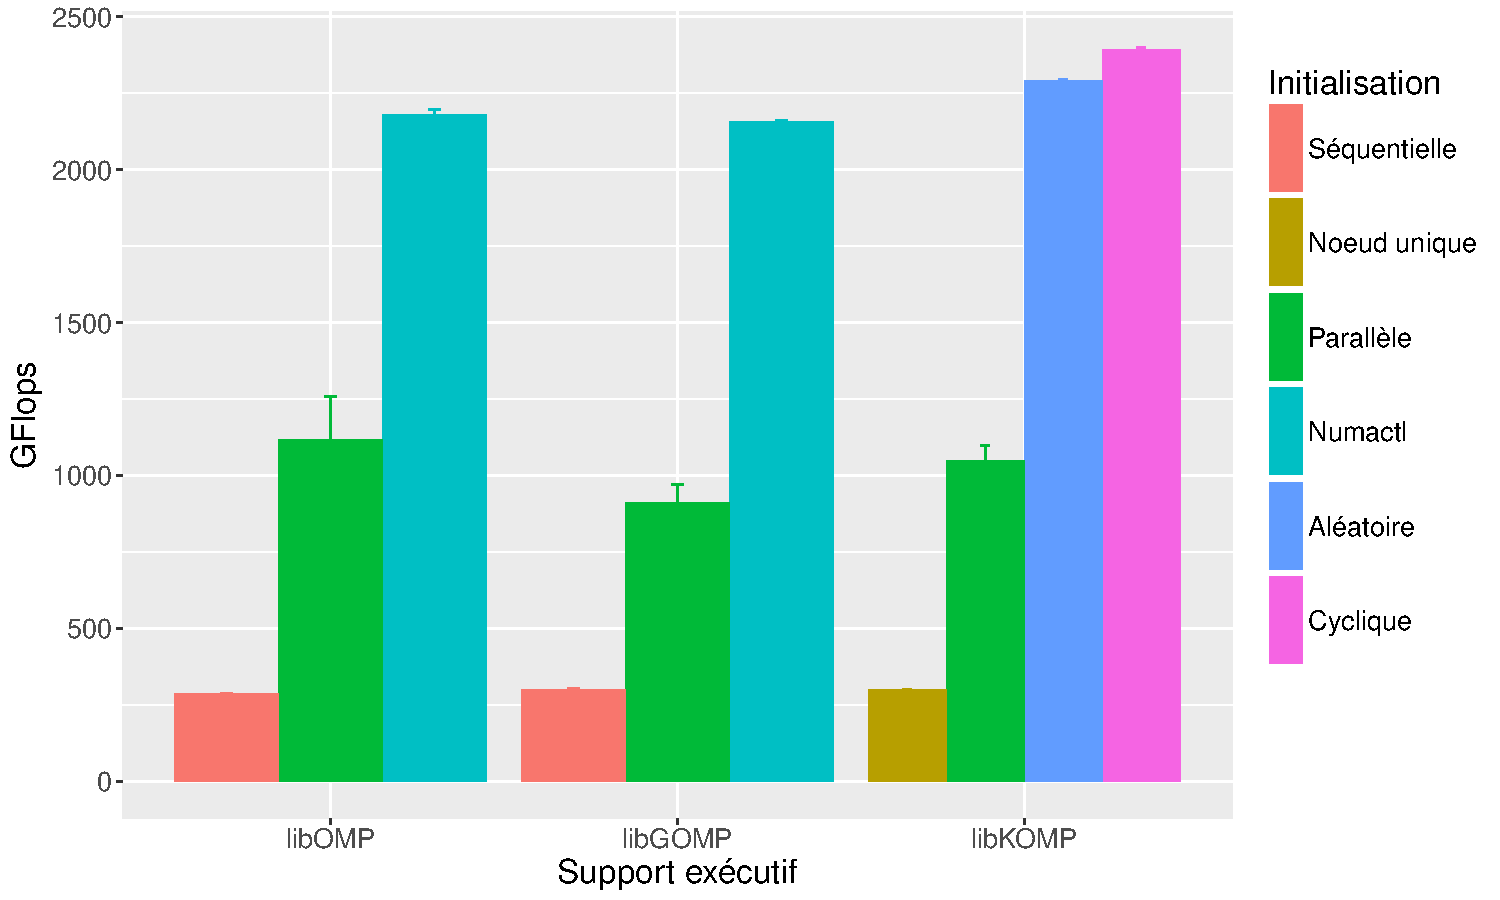
\includegraphics[width=\textwidth]{graph_distrib_data_idchire}
  \caption{Performances des différentes stratégies pour Cholesky en fonction de la distribution de données (N=32768, BS=512)}\label{fig:contribs:perf_eval:distrib-idchire}
\end{figure}

\subsubsection{Impact de l'affinité, et étude comparative des stratégies}

\begin{figure}[ht]
  \centering
  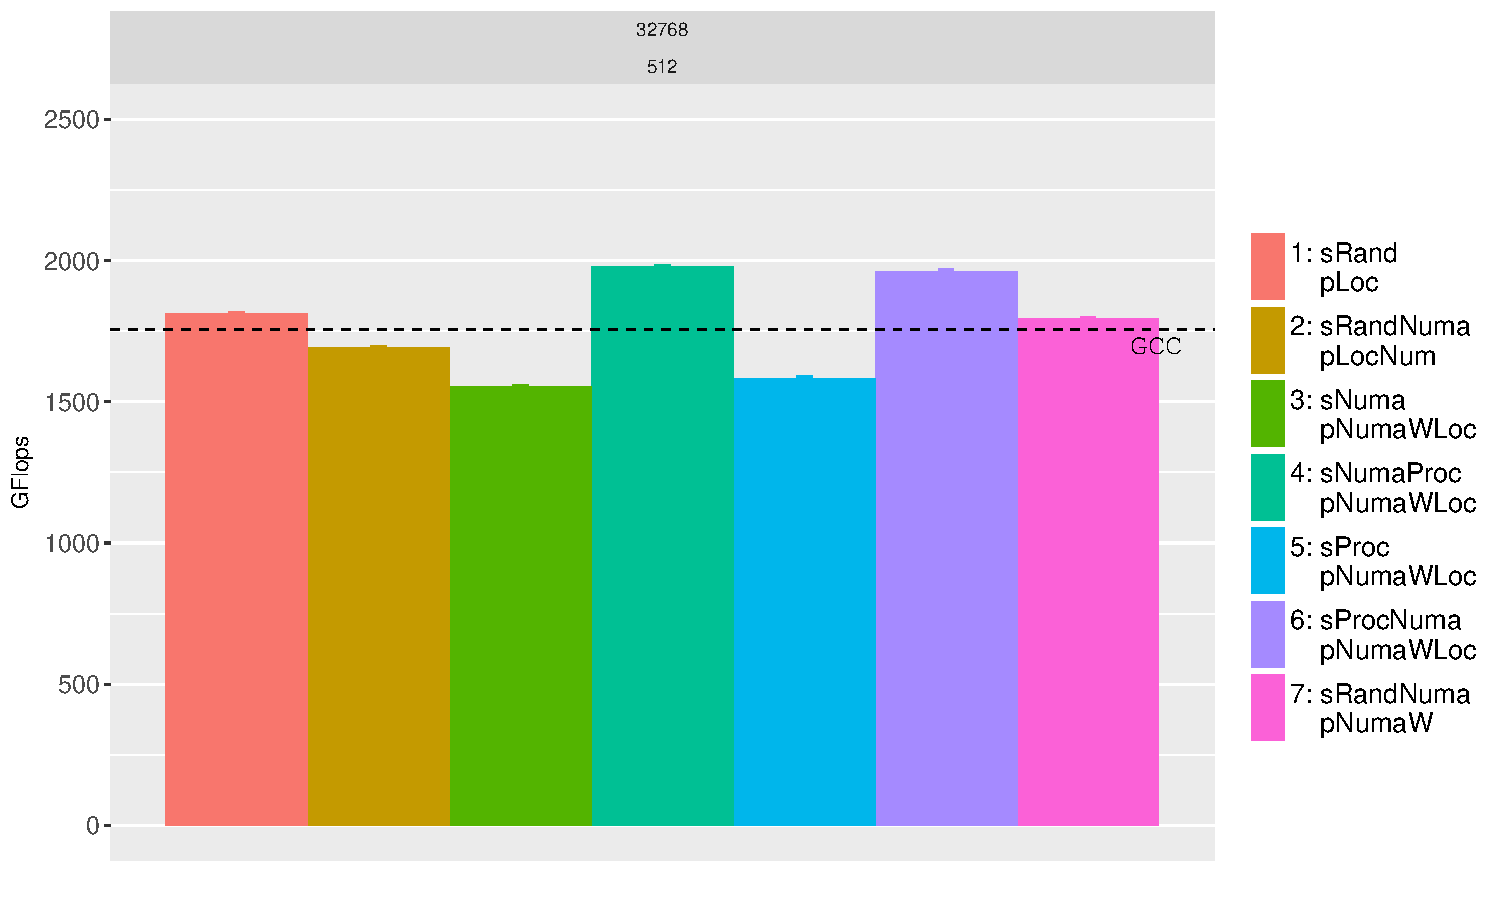
\includegraphics[width=\textwidth]{graph_all_strat_idchire}
  \caption{Performances des différentes stratégies pour Cholesky (N=32768, BS=512)}\label{fig:contribs:perf_eval:eval-strategies}
\end{figure}

\begin{figure}[ht]
  \centering
  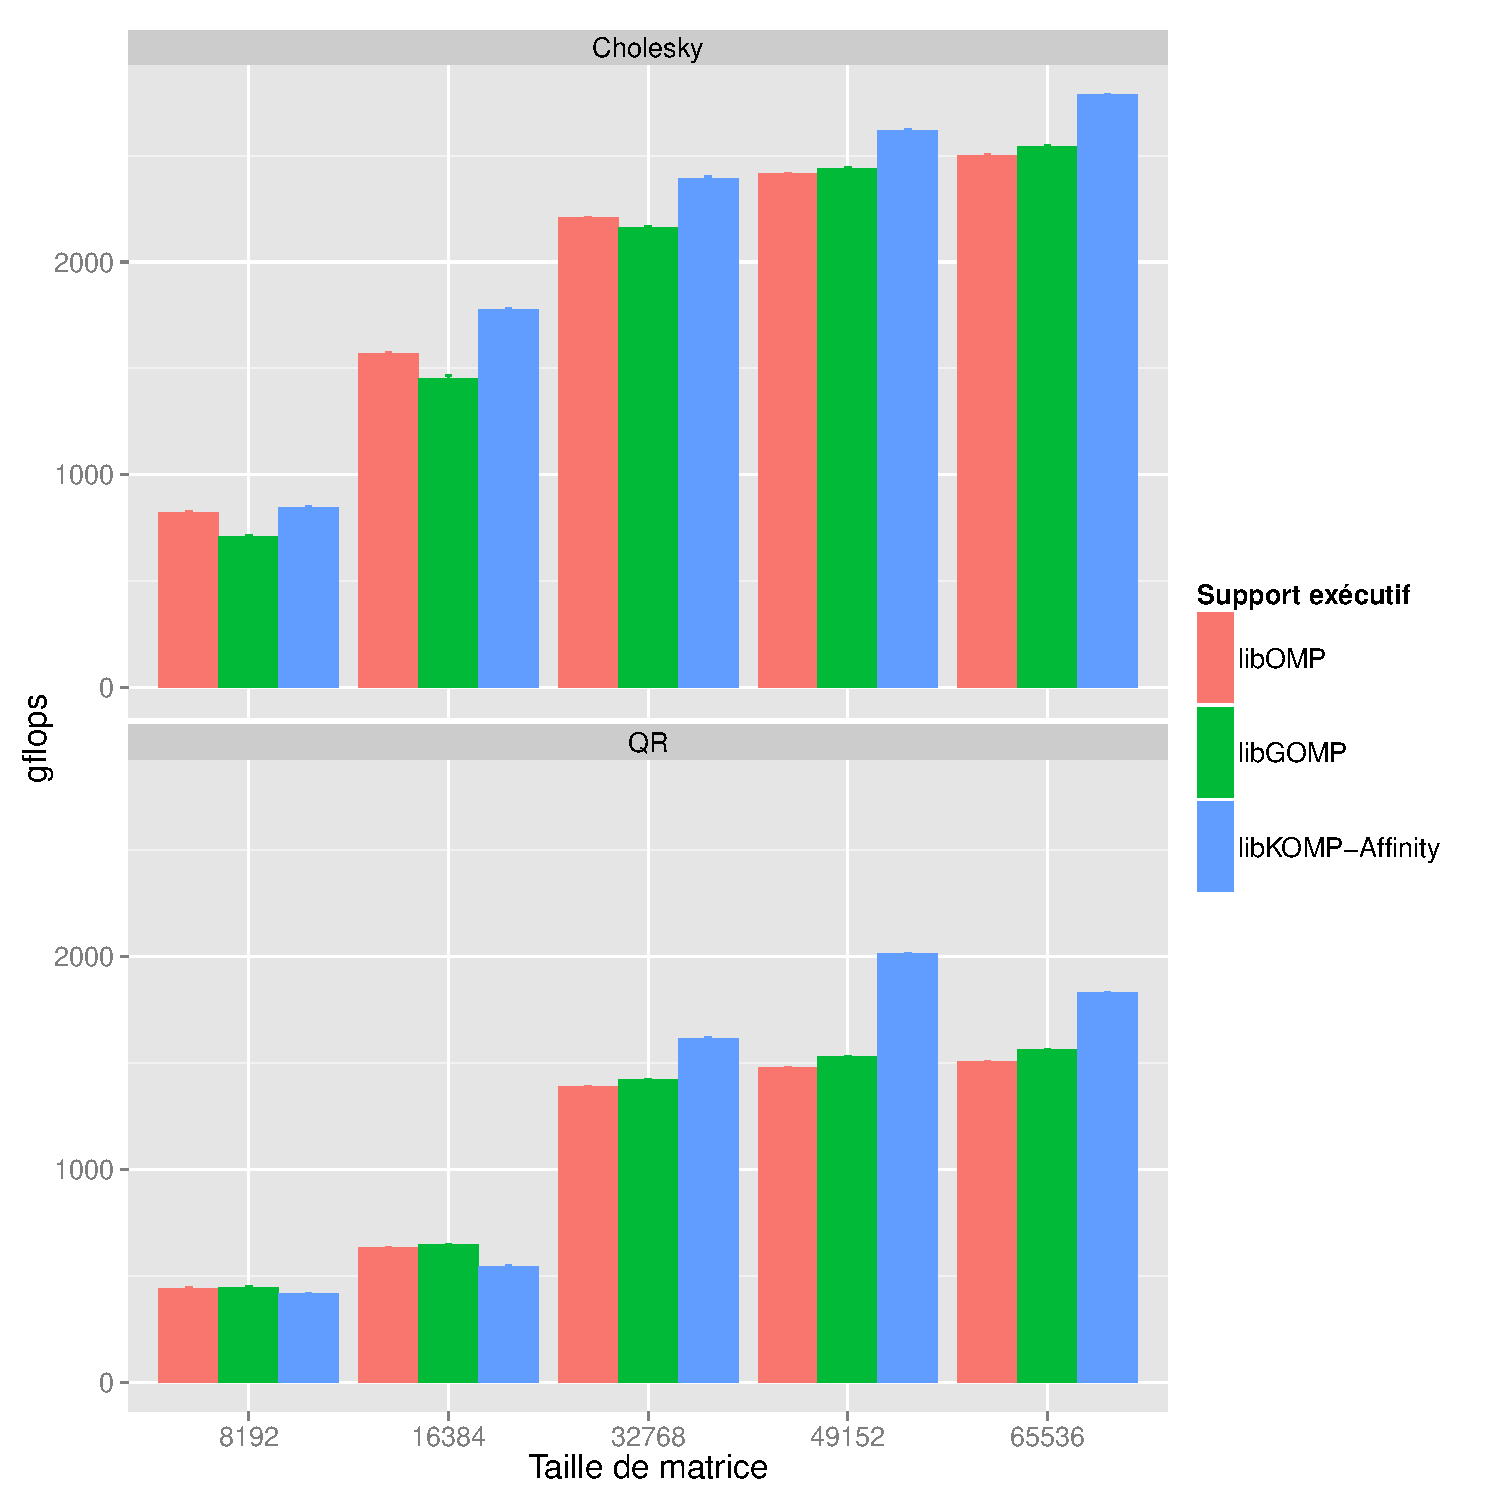
\includegraphics[width=\textwidth]{graph_details_qr_cholesky_idchire}
  \caption{Comparaison de trois stratégies sur QR et Cholesky, en fonction de la taille de matrice}\label{fig:contribs:perf_eval:eval-qr-cholesky}
\end{figure}

\begin{todo}
GRAPHE : 5.5.2, Cholesky : (presque non-)impact stratégies affinité sur brunch/idkat
\end{todo}

\subsubsection{Affinité vers des cœurs}

\begin{figure}[ht]
  \centering
  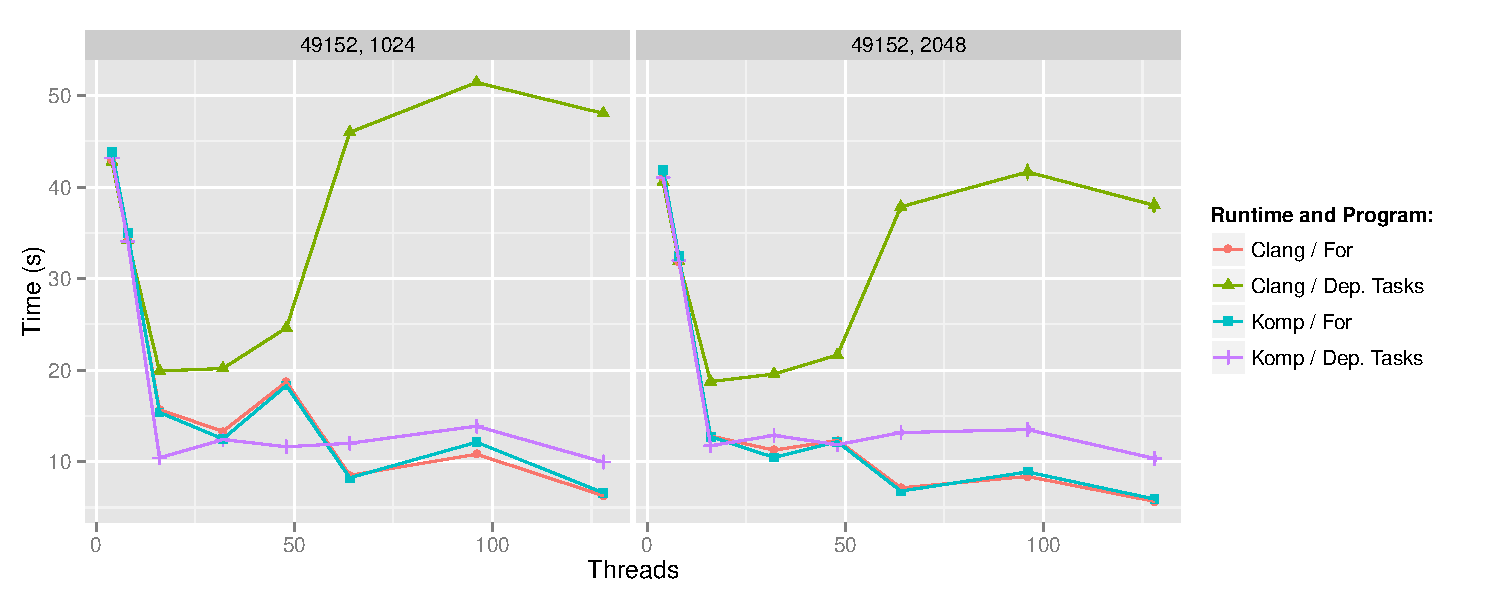
\includegraphics[width=\textwidth]{jacobi_scale_iomp_komp}
  \caption{Performances de Jacobi en fonction de la version et du support exécutif}\label{fig:contribs:perf_eval:eval-jacobi}
\end{figure}

\subsection{Portage dans un autre support exécutif}\label{sec:contribs:perf_eval:libkomp}

\subsubsection{Description}

\subsubsection{Évaluation}

/!\ pour ces xp les versions de gcc/clang ont changé, ainsi que les BLAS !

\begin{todo}
  Il faut aussi comparer ça au simulateur. Peut être plus simplement faire une section à part.

  Vu que c'est principalement effectué avec le nouveau libkomp, peut être mettre ça dans une section suivant celle du "portage" vers le runtime intel.

  À discuter de où on met ça...
\end{todo}


